\documentclass[11pt,a4paper]{article}

\usepackage[plain]{fullpage}
\usepackage{graphicx}
\usepackage[hidelinks]{hyperref}
\usepackage{caption}
\usepackage{subcaption}
\usepackage{wrapfig} 
\usepackage{enumitem}
\usepackage{amsmath}

\newcommand{\HRule}{\rule{\linewidth}{0.5mm}}

\begin{document}
\begin{titlepage}
\begin{center}

~\\[3cm]
{\Huge Status of the Voyager project}\\[1cm]

{\large TTT4234 Space Technology I}\\[1.5cm]

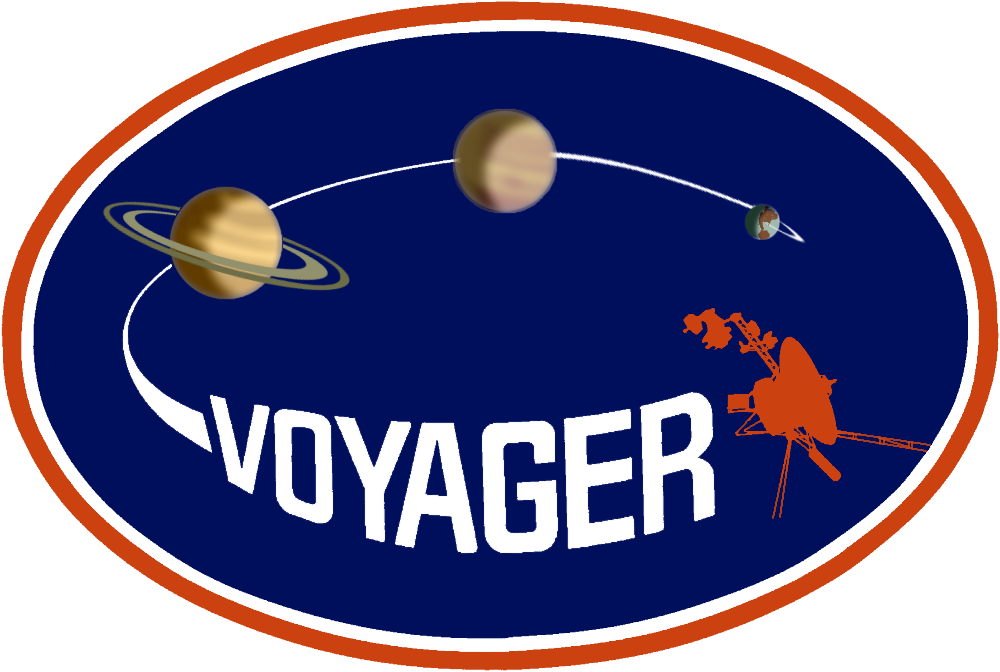
\includegraphics[width=0.4\textwidth]{./voyagerlogo}~\\[1.5cm]


% Author and supervisor
{\large Antonio Maria Franques Garcia\\ \texttt{antoniof@stud.ntnu.no}}\\[1cm]
{\large Trondheim, \today}


\vfill

% Bottom of the page
\textsc{\large Department of Electronics and Telecommunications} \\
\textsc{\large Norwegian University of Science and Technology}

\end{center}
\end{titlepage}
\clearpage
\tableofcontents
\clearpage

\section{Introduction}
\textbf{What is this essay about and what do we pretend with it?}
The goal of this essay is, at the end, to explain which are the current and future studies carried out by both probes that constitute the Voyager project, the Voyager 1 and Voyager 2. For reaching that aim we will first introduce to the reader the necessary knowledge about the Voyager project, as we consider that it is the only way to understand which are the physical limitations or constraints that are defining and will define the possibilities of their missions.

\section{The Voyager project}
\begin{wrapfigure}{r}{0.5\textwidth}
  \begin{center}
  \vspace{-20pt} 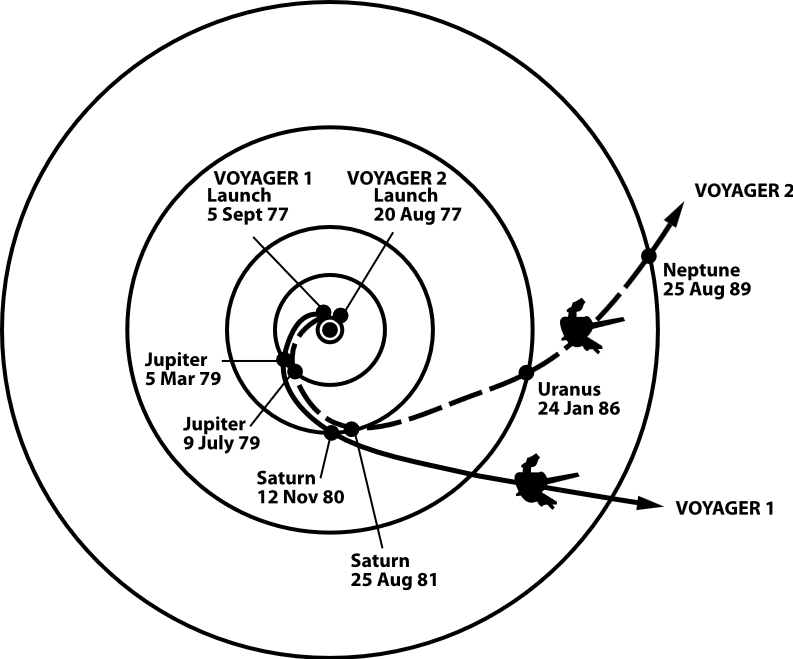
\includegraphics[width=0.48\textwidth]{./voyagerpath}
  \end{center}
  \vspace{-5pt}
  \caption{}
  \vspace{-10pt}
\end{wrapfigure}
\textbf{First of all, what is the Voyager project?}
The american project Voyager (originally part of the Mariner program), financed by the National Aeronautics and Space Administration (NASA), consisted in the launch (by Titan-Centaur rockets from Cape Canaveral) and further monitoring and control of two non tripulated probes to the space, the Voyager 1 and 2.
\\\\
Although for both probes the initial goal was to obtain new information about two of our neighbours (Solar System) planets, Jupiter and Saturn, there was a big difference between the Voyager 1 and Voyager 2: the Voyager 2 would additionally try to explore Uranus and Neptune. The moment chosen for their launches (20th of August of 1977 and 5th of September of 1977, respectively for Voyager 2 and 1) was due to a pretty rare planet alignment (occurs only once every 175 years) that would let them use the recently discovered gravity assist maneuver. This technique consists on changing and accelerating the original path of the spacecraft by the closeness to the gravity field of a planet (or other astronomical object), saving that way propellant and time. Both probes used that maneuver for approaching Saturn via Jupiter, but additionally the Voyager 2 used that technique for reaching Uranus via Saturn and later on Neptune via Uranus (see Figure 1). Meanwhile, the Voyager 1 kept his own trip straight towards the limits of the Solar System. The final result of these maneuvers made that both probes are travelling nowadays in almost 90 degrees difference directions. Taking advantage of this planet alignment both probes could save their own propulsors for small corrections on their trajectories instead of having to use it mainly on big direction changes.
\\\\
It must be said that initially NASA gave to the mission less founds than expected, it is for that reason that the Voyager probes were originally built just for performing an intense study of Jupiter and Saturn. Nevertheless, as we have mentioned before, for the Voyager 2 it was chosen a trajectory that could let it continue its trip (in case that NASA would provide more founds) towards Uranus and Neptune (taking advantage of the planet alignment). It is also good to know that there was a previous NASA’s project that provided important data and experience for the design and construction of the Voyager project, it was the Pioneer program. The Pioneer 10 and 11, two probes launched 5 years before the Voyagers, had the aim of obtaining information about Jupiter and Saturn; they were the firsts human-created objects reaching that distance.

\section{Accomplishments}
\textbf{What kind of information have they (the probes) given us so far?}
In their first mission, study of Jupiter and Saturn, the probes obtained very important information for a better understanding of the Solar System; enough information as to keep carrying out several years of further research. Some of these important discoveries were: 
\begin{itemize}
\item Active volcanoes on Jupiter's moon, Io (this was the greatest unexpected discovery at the flyby of Jupiter, since it was the first time that volcano activity were seen in another Solar System body)
\item Rings around Jupiter
\item Additional moons around Jupiter (Adrastea, Metis and Thebe)
\item New data of the Jupiter Great Red Spot
\item New data of the Saturnian moon Titan
\item Jupiter's complex cloud forms, winds and storm systems
\item Saturn temperature difference between uppermost and deepest pressure levels 
\item Saturn’s rings were found to be formed by millions of small ice particles, to have enigmatic braids, kinks and to be accompanied by myriad of "ringlets"
\end{itemize}
The success of this first mission led NASA to invest more money on the Voyager program. Therefore, the Voyager 2 could continue its monitored trip to Uranus and Neptune and the Voyager 1 keep his straight trip to the boundaries of the Solar System. The mission was then renamed as "Voyager Neptune Mission". This next stage brought lots of new information about the Ice Giant planets (Uranus and Neptune), some of these were:
\begin{itemize}
\item Characterization of the magnetic field around Uranus. It was found that the inclination of this planet has effects on the tail of its magnetic field.
\item Discovery of 11 additional Uranus moons (Cordelia, Ophelia, Bianca, Cressida, Desdemona, Juliet, Portia, Rosalind, Belinda, Perdita and Puck)
\item Discovery of 3 rings around Neptune
\item Furhter characterization of the Uranian ring system. It was found that the radiation of its rings has an intensity similar to the rings of Saturn
\item Discovery of 6 additional Neptune moons
\item Discovery of auroras on Neptune
\end{itemize}
After the Voyager 2 had overtaken Neptune, now with both probes going out of the solar system (after more than 12 years travelling through it), the project was renamed as "Voyager Interstellar Mission", where both probes kept studying the fields and particles that they found on their ways. The main goal of this mission would be to reach the Heliopause, which is the limit between the area under the Sun influence and the interstellar space. Basically is the place where the electrical particles produced by the Sun (solar wind) shock with those coming from the interstellar space (see Figure 2). The Voyager 1, which although it was launched later than its sister Voyager 2 it finally overtook it, reached and crossed the Heliopause on August 2012, becoming the first manmade object leaving the Solar System. At this point it must be said that for reaching the Heliopause, the Voyager 1 had to first cross the Termination Shock (December 2004), which is the point where the solar wind decrease notoriously its speed, and travel all through the Heliosheath, which was unknown how long would it take to cross; it was finally 7 years and 8 months. Meanwhile, the Voyager 2 crossed the Termination Shock in September 2007 and it is expected to have reached the Heliopause by 2016. Since the radial distance to the Sun where the Voyager 1 crossed the Termination Shock was not the same than where the Voyager 2 did, it was discovered that the Solar System is asymmetrical.
\\
\begin{figure}[hb]
  \centering
  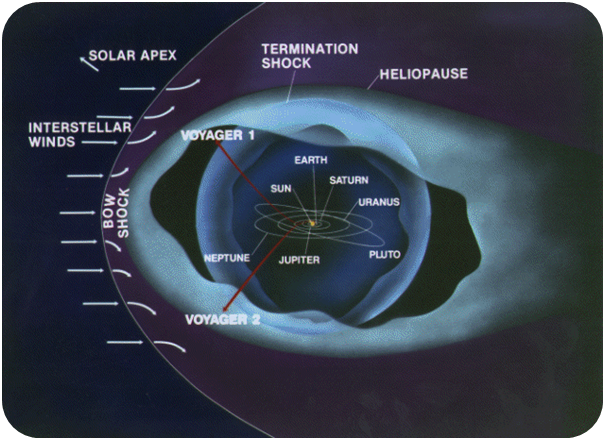
\includegraphics[width=4in]{./heliosphere}
  \caption{}
\end{figure}

\section{Instruments on board}
\textbf{How did/do they gather all that information?}
Both Voyager 1 and Voyager 2 have the same structure and weight, which is around 800 Kg. Each probe is equipped with a large number of scientific instruments, electronic components as well as with computer programming (Computer Command Subsystem) for, amongst other purposes, autonomously fixing many kinds of possible failures.
\\\\
Note: Since the communications and command instructions from earth would take several hours to reach the probe it was mandatory to design and install this autonomous fault protection system. That way the probes could solve their own failures in a matter of seconds or minutes. 
\\\\
A roughly detailed list of the scientific instruments on board is written in the following subsections.

\subsection{Imaging Science Subsystem (ISS)}
\begin{wrapfigure}{r}{0.5\textwidth}
  \vspace{-10pt}
  \begin{center}
    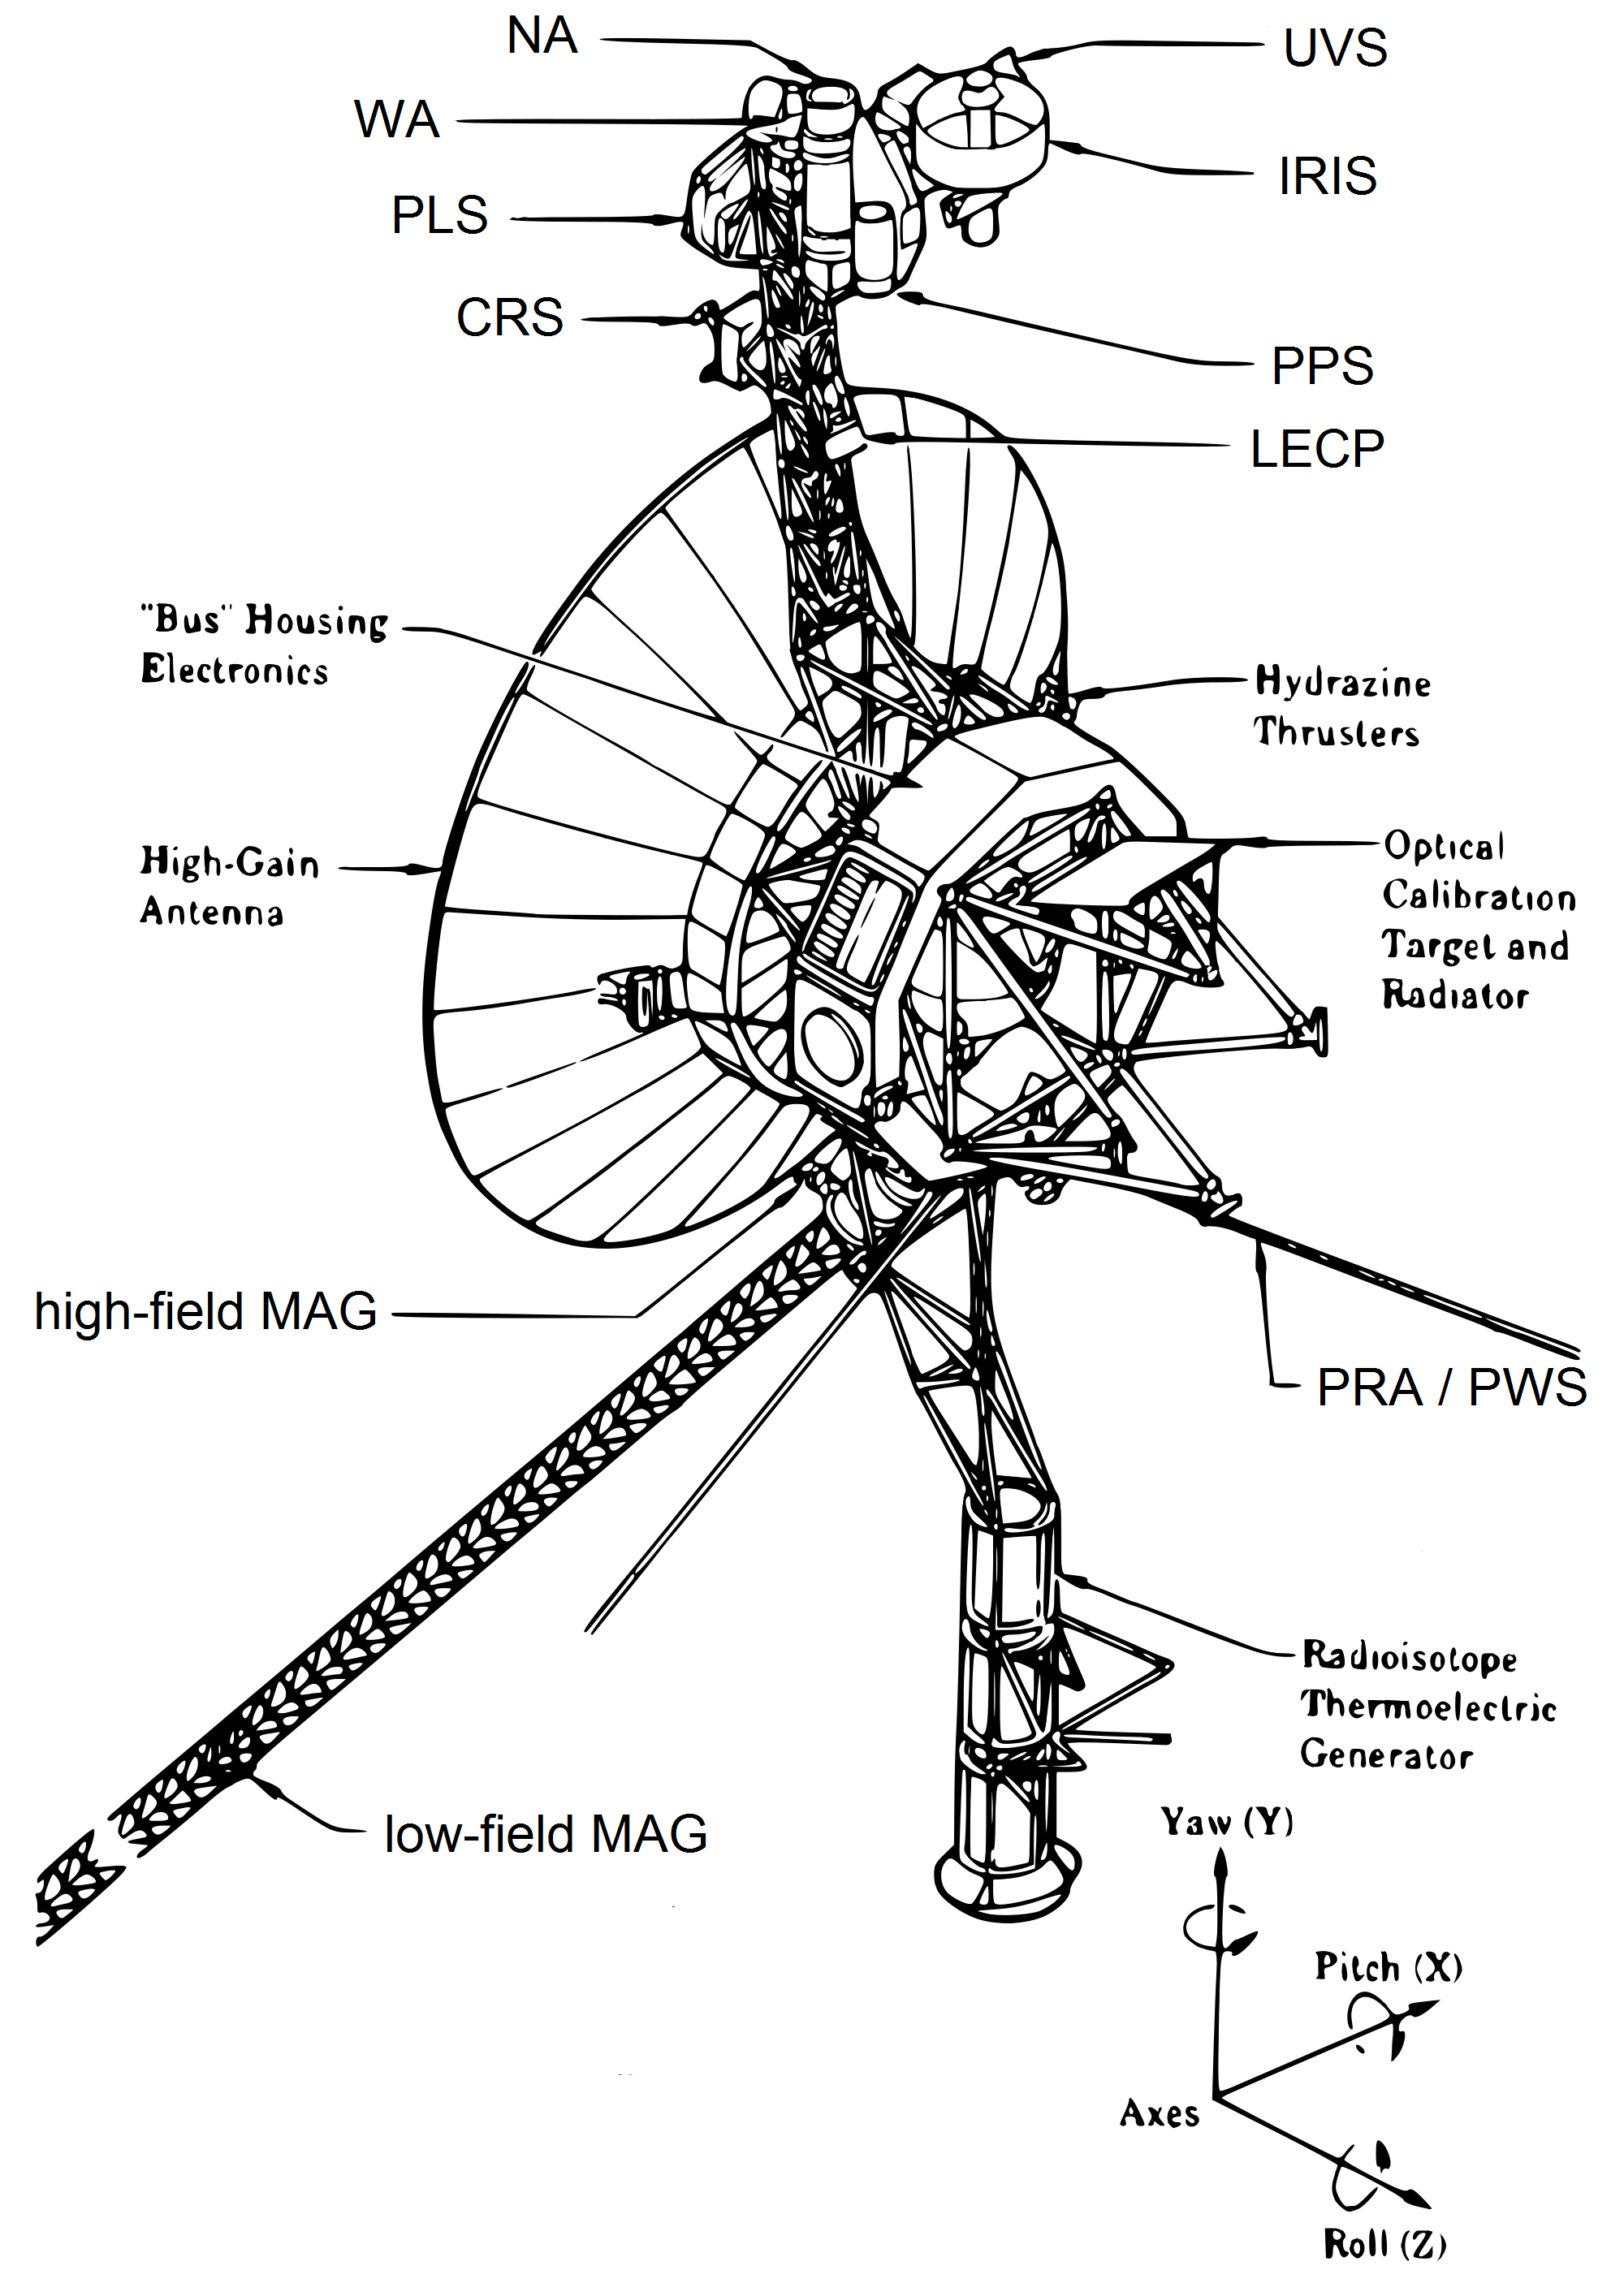
\includegraphics[width=0.48\textwidth]{./voyagerstructure}
  \end{center}
  \vspace{-30pt}
  \caption{}
  \vspace{0pt}
\end{wrapfigure}
There are two cameras in order to take pictures in the visible frequencies range of the spectrum: the Wide Angle Camera (WA), used for capturing more area in a single picture, and the Narrow Angle Camera (NA), used for capturing a reduced, but in high detail, area picture. The NA has a resolution such that it could read a newspaper at a distance of 1 Km. These cameras were used with several aims, some of them were: capturing the motion of Jupiter and Saturn as well as their cloud distributions, capture the orientation of their spin axes, capture of spots in their surfaces (like the Jupiter’s Great Red Spot), observation of their satellites, etc. More information about it can be found in \cite{ISS}.

\subsection{Photopolarimeter Subsystem (PPS)}
It is used for measuring the composition and surface texture of the observed bodies (Jupiter, Saturn, Uranus and Neptune) as well as for gathering information about theirs atmosphere (scattering and density). For doing that it detects how the light change when is reflected by the body. For discerning different kinds of light it uses eight different filters. See \cite{PPS}.

\subsection{Infrared Interferometer Spectrometer and Radiometer (IRIS)}
This instrument provides the temperature of the observed body (planets and satellites) and the composition of its atmosphere. Additionally it was used for determining the size of the particles that composes the Saturn’s rings. See \cite{IRIS} for more information.

\subsection{Ultraviolet Spectrometer (UVS)}
As well as the IRIS instrument it provides information about the atmosphere composition of the observed body. It is also used for detecting some of the physical processes that release ultraviolet radiation. See \cite{UVS}.

\subsection{Radio Science Subsystem (RSS)}
This instrument takes advantage of the radio waves used for the communication with the earth for measuring densities, temperatures and atmosphere pressures of the observed body (planets and satellites). It also helps on the estimation of the planetary rings composition and dimensions. See \cite{RSS}.

\subsection{Planetary Radio Astronomy (PRA)}
It measures the radiofrequency sent out by the Sun as well as by the Gas Giants, Jupiter and Saturn. For doing that it uses a radio receiver sweeping all frequencies in the range. See \cite{PRA}.
\subsection{Plasma Wave Subsystem (PWS)}
Analogous to the PRA but working on a different range of frequencies. It was used in the study of Jupiter and Saturn magnetospheres. Both instruments (PWS and PRA) are placed one beside the other. See \cite{PWS}.

\subsection{Magnetometer (MAG)}
As we can imagine by its name it measures the magnetic field produced by the observed planets (Jupiter and Saturn) as well as by the Sun (interaction between the solar wind and the planet's magnetosphere). This instrument is actually separated and located into two different parts, the low-field MAG and the high-field MAG. The low-field MAG is located on a thirteen meters long bar structure that was initially fold (but instantly deployed once the probe reached the outer space). See \cite{MAG}.

\subsection{Plasma Spectrometer (PLS), Low Energy Charged Particle Instrument (LECP), Cosmic Ray Subsystem (CRS)}
These three instruments, each one independent to the others, are used for detecting particles charged in a different levels of energy. The PLS can detect ions from 10 eV to 6 KeV and electrons from 4 eV to 6 keV, its purpose is focused on the properties (density, temperature and speed) of the solar wind but also any other kind of plasma. The LECP can detect ions from 10 keV to 150 MeV and electrons from 10 keV to 10 MeV, it focuses on differentiating fluxes and compositions of ions and electrons. Finally the CRS focuses on the cosmic rays nuclei (from 1 MeV/n to 500 MeV/n), although it also measures electrons from 3 MeV to 110 MeV. See \cite{PLS,LECP,CRS}.

\subsection{Additional information}
The location of all these instruments in the structure of the probes can be seen in Figure 3. It must be said that although in the Figure we see the naked structure of the probe, they both (Voyager 1 and 2) covered their most sensible instruments with a very protective shield against radiation emissions. It was imperatively needed for the flyby to the Jovian system since the radiation of this planet is (at the flyby distance where the two probes were) the equivalent to a thousand times the human lethal dose. 
\\\\
Besides the thrusters used for correcting the probes trajectories, they both have several thrusters based on a three axis basis used for different purposes (it is called the attitude control). Some of these are:
\begin{itemize}
\item To stabilize the spacecraft as much as possible during the exposure time needed for taking the pictures
\item For Gyro operations (used for a good calibration of the Magnetometers)
\item For pointing its other instruments towards the selected target with an accuracy of a tenth of a degree (also with the help of the rotating platforms)
\end{itemize}
The gyroscopes installed on board provide the angular motion needed for reaching that aim. This subsystem is called AACS (Attitude and Articulation Control Subsystem).


\section{Power subsytem}
\textbf{How do they obtain the necessary energy for collecting, treating and sending that information to the earth?}
The electrical power of the spacecraft (which is the same in both probes) is provided by three Radioisotope Thermoelectric Generators (RTG) mounted in series, which produced, at the moment of their launch, a total of 475 Watt at 30 Volts of Direct Current (DC). Such a power supply would be the equivalent to one third of an average residential house. Its operation is the following: inside every RTG there is a determined quantity of plutionium-238, this radioactive material produces (due to its degeneration) a continuous flow of alpha particles, which as a consequence of their hit with various materials produce a huge quantity of heat (atomic motion). This heat is finally transformed into electricity by the Seebeck effect (based on temperature differences). See \cite{seebeckwikipedia} and \cite{RTG} for more information.
\\\\
Since Plutionium-238 (the fuel used for the RTGs) decays with a half-life of 87.7 years, the RTGs lose 0.79\% of their power per year. Also the part that converts heat into electricity suffers degradation, which implies that the real output power of the RTGs are lower than its calculated level. The more the power decreases the more loads (instruments) must be turned off in order to avoid exceed the supply demand. In 1989 after Voyager 2 observed the last of the Gas Giants and started its trip to the outer Solar System, the mission engineers powered down all non-essential systems in order to save as much energy as possible. It is expected that the RTGs will supply enough power as to keep some operations of the Voyager 1 and 2 until at least 2025 and 2020, respectively.

\section{Communication with Earth}
\textbf{How is all that information sent from/to the probes?}
The probes have maintained a constant communication with the earth, not only from the probes towards the earth (downlink) but also the instructions from earth towards the probes (uplink). For fulfilling such an aim, both sides of the communication should overcome the huge limitations of the distance (remember from the transmission law that the power of an electromagnetic wave decreases at the reason of the squared distance) and noise addition. How did/do they do it?
\\\\
On the probes side, both Voyager 1 and 2 are equipped with two antennas: a high-gain (very directive) antenna and a low-gain (almost isotropic) antenna. The diameter of the high-gain antenna reflector is 3.7 meters and it supports the X (7.0 to 11.2 GHz) and S (2.0 to 4.0 GHz) microwave frequencies bands. The low-gain antenna is placed on the sub-reflector of the high-gain antenna, which is a Cassegrain type (see Figure 4.a) and it is used in case that the high-gain antenna cannot properly point the Earth. The downlink is placed in the X band at a central frequency of 8.4 GHz and the uplink is in the S band at a central frequency of 2.3 GHz. Although at the distance of Jupiter (the first target of the mission) the data rate was about 115 Kbps, it had already decreased to the half at the distance of Saturn (the immediately next target).
\\\\
Besides the antennas, the communication system of the Voyagers includes: a variety of signal amplifiers (which gives up to 23 Watt of power for transmission), up and down converters (due to the fact that all the signal treatment is done at intermediate frequency but the transmitted and received signal is at high frequency), Phase Locked Loops (in order to generate the carrier used for multiplexing and demultiplexing the signal), etc.
\\\\
On the earth side, different techniques have been developed as time goes by for trying to distinguish such a weak signal coming from the probes amongst all the non-desired rest (noise). The most important two are:  
\begin{itemize}
\item Increasing the diameter of the receiver's parabolic dishes (reflectors)
\item Combining the signal received by different antennas strategically placed (antenna array). See fore example Figure 4.b
\end{itemize}
By these two techniques we obtain a better effective receiver area and directivity (pointing) of the antennas and hence a better quality of the desired signal. Additionally, several receiver antenna parks are placed over the world (California, Madrid and Canberra) in order to ensure that at least there is always one of them facing the probes; it is called the Deep Space Network (DSN).
\\\\
When the probes are not able to send data to Earth (because maybe the communication system is busy) they record the content (thanks to the Digital Tape Recorder) and send it afterwards when the communication is available again. They can record up to 69.63 Kbytes (a millionth part of our daily computer hard disk drives). There were installed many reader headers in both probes (as a safety measure) due to the fact that every day the tape is recorded, rewind and resumed several times. The Plasma Wave Subsystem (PWS) makes use of these record tapes due to its high-rate obtainment of the data (however in the case of the Voyager 2 there is no need for it anymore, as a consequence of a failure in the PWS in June 2002).

\begin{figure}[hb]
        \centering
        \begin{subfigure}[b]{0.4\textwidth}
                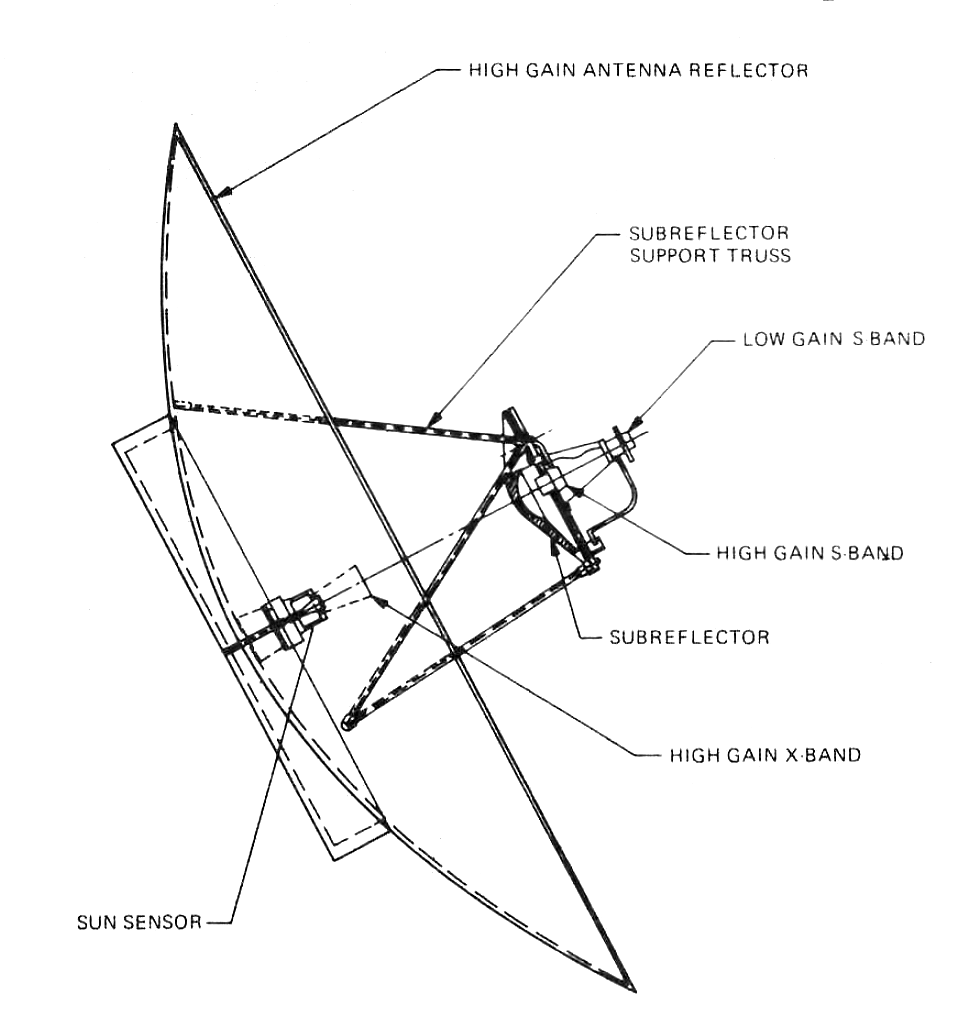
\includegraphics[width=\textwidth]{./voyagerantenna}
                \caption{}
        \end{subfigure}%
        ~ \quad %add desired spacing between images, e. g. ~, \quad, \qquad, \hfill etc.
          %(or a blank line to force the subfigure onto a new line)
        \begin{subfigure}[b]{0.4\textwidth}
                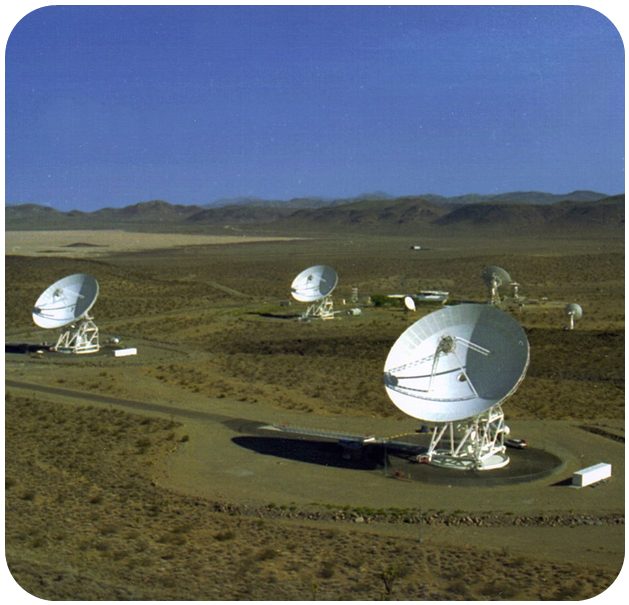
\includegraphics[width=\textwidth]{./antennaearth}
                \caption{}
        \end{subfigure}
       
        \caption{}
\end{figure}

\section{Current and future missions of the project}
As we have mentioned at the end of the Accomplishments section, the probes are nowadays farther than anything ever previously made by humanity, however since most part of the instruments had to be powered down (mainly because of the power supply but also because of some failures) and the bitrate of the communication with Earth has notoriously decreased due to its larger distance and noise addition, we can only get a few kinds of data about its actual environment, the interstellar space.

\subsection{Current instrumentation}
The operating instruments remaining in the Voyager 1 are:
\begin{itemize}
\item Low Energy Charged Particle Instrument (LECP)
\item Cosmic Ray Subsystem (CRS)
\item Magnetometer (MAG)
\item Ultraviolet Spectrometer (UVS)*
\item Plasma Wave Subsystem (PWS)
\end{itemize}
Let's notice that there is an important instrument missing in the Voyager 1, The Plasma Spectrometer. It is due to its failure in 1980, when the probe was near Saturn.
\\\\
*Note: Although this instrument was initially expected to be powered down at 2000 it is still operative due to a group of interested scientist that requested to keep investigating some unexpected Ultraviolet levels detected in the wind.
\\\\
And in the case of the Voyager 2 are: 
\begin{itemize}
\item Low Energy Charged Particle Instrument (LECP)
\item Cosmic Ray Subsystem (CRS)
\item Magnetometer (MAG)
\item Plasma Wave Subsystem (PWS)**
\item Plasma Spectrometer (PLS)
\end{itemize}
**Note: Only partially working due to its failure on June 2002.
\\\\
These instruments are still letting that five investigation teams collect enough data as to keep the mission alive.

\subsection{Current mission}
On the one hand, the current mission of both Voyager probes (The Interstellar Mission) consisted (in the case of the Voyager 1) and consists (in the case of the Voyager 2) on crossing and getting information about the surroundings of the Heliopause, this is already done in the case of the Voyager 1, since the scientists of the mission officially reported its arrival to the interstellar space***. On the other hand, the second part of the mission consists on gathering as much information as possible about the interstellar space (the area where the dominating gases come from other stars). Why is so important to reach the interstellar space? Because it is only in the abscence of the solar influence (magnetosphere) where authentic data of the interstellar space can be obtained, e.g. density and temperature of its plasma. These measures are expected to reveal new discoveries and knowledge about the interstellar space, and thereby about the origin of all times (see \cite{historicjourney}). An exemple of that is the assumption that for several years the scientific community had about the existance of the Sun's bow shock and that Voyager 1 took apart when it crossed the Heliopause; it revealed that such assumption was erroneous.
\\\\
***Note: How did the scientists know that the Voyager 1 had already reached the interstellar space if its Plasma Spectrometer was not operative? As we can see in \cite{edstone} and \cite{howdoweknow}, it was a mix of good luck and good scientific team. Although there were some previous hints, the determining fact was the Sun burst (burst of solar wind and magnetic fields) occurred around March 2012. It took 13 months for this burst to arrive to the Voyager 1 but when it did it could measure (thanks to the Plasma Wave Instrument) the vibration of its surrounding plasma and thus determine that the density of it (more than 40 times denser than the outer layer of the Heliosphere) was that corresponding to the interstellar space.

\subsection{Future missions}
\textbf{What can we still expect to obtain from the probes?} Although the power of the emitted signals of both Voyager 1 and 2 will do nothing but keep decreasing it is still expected to receive a daily bunch of data. In the case of the Voyager 1, from the interstellar space, and in the case of the Voyager 2 from both Heliosphere and interstellar space. Let's not forget that this latest  (Voyager 2) has its Plasma Spectrometer still operating (in contrast to the Voyager 1) and therefore it will keep supplying more accurate data about its trip across the Heliosheath and hopefully later on also about the interstellar space.
\\\\
The following instruments are expected to still be operating by 2020,
\begin{itemize}
\item Voyager 1: Low-Energy Charged Particles, Cosmic Ray Subsystem, Magnetometer and Plasma Wave Subsystem.
\item Voyager 2: Low-Energy Charged Particles, Cosmic Ray Subsystem, Magnetometer, Plasma Wave Subsystem and Plasma Subsystem.
\end{itemize}
~\\
Even at the end, once the power supplied by the RTGs are not enough as to maintain any single instrument in either probes or to keep a communication with the earth, there will still be a last mission for the two of them: the hope to its contact with any kind of other life. For this reason both probes contain a Golden Record, a gold protected phonograph disc with information about their origin, the Earth. See \cite{goldenrecord} for further information.

\section{Conclusion and personal opinion}
\textbf{What have we learned from this essay?}
as we have seen throughout the content of this essay, the Voyager project has been a non-stop series of accomplishments and new discoveries. Travelling farther than anything or anyone in the history of our existence and moreover reaching the door of the interstellar space. Just for having an idea of the importance of the Voyager project for the knowledge of our own Solar System, it is enough to say that both probes have sent to the Earth more than five trillion of bits with relevant scientific data, discovered twenty-two new satellites (amongst the four studied planets), discovered that Saturn's rings are made by million of tiny ice particles, discovered the active volcano activity in Io, discovered the Neptune's rings and characterized the Uranus magnetic field.
\\\\
It is clear from here that this mission, after more than 37 years since its beginning (and still counting), has set a very high standard on the history of the Space program.
\\\\
My personal opinion about the ending of its journey is, probably due to a mix of ignorance and hope, that in the inmensity of the Space there will be someone at some moment with the ability necessary as to not only capture either of the probes but also to understand the instructions given on the Golden Record as to successfully read its content and thus discover of our existance. Of course it could also be that it would be too late, maybe we are not here anymore as to receive their reply or visit, but at least is exciting for oneself to imagine these probes travelling amongst stars, being our most remote embassadors.
\\\\
The writing of this essay has provided me, throughout all the hours spent on its research, its understanding and its summarizing, a very good overview of the Voyager project, allowing me from now on to not only follow but also deeply appraise all incoming news and data about it.


\begin{thebibliography}{99}
\bibitem{overview} Spacecraft overview, JPL/NASA Voyager project official webpage, \url{http://voyager.jpl.nasa.gov/spacecraft/index.html}

\bibitem{didyouknow} Voyager facts, JPL/NASA Voyager project official webpage, \url{http://voyager.jpl.nasa.gov/mission/didyouknow.html}
\bibitem{lifetime} Spacecraft lifetime, JPL/NASA Voyager project official webpage, \url{http://voyager.jpl.nasa.gov/spacecraft/spacecraftlife.html}
\bibitem{interstellar} Interstrellar mission, JPL/NASA Voyager project official webpage, \url{http://voyager.jpl.nasa.gov/mission/interstellar.html}
\bibitem{edstone} Ed Stone (Project Leader Scientist) talks about Voyager's interstellar arrival, JPL/NASA Voyager project official webpage, \url{http://www.jpl.nasa.gov/interstellarvoyager/q-and-a/}
\bibitem{howdoweknow} How do we know when Voyager reaches interstellar space?, JPL/NASA Voyager project official webpage, \url{http://www.jpl.nasa.gov/news/news.php?release=2013-278}
\bibitem{historicjourney} Historic Journey Into Interstellar Space, JPL/NASA Voyager project official webpage, \url{http://www.jpl.nasa.gov/news/news.php?release=2013-277}
\bibitem{voyagerwikipedia} The Voyager program, Wikipedia, \url{http://en.wikipedia.org/wiki/Voyager_program}
\bibitem{voyager1wikipedia} Voyager 1, Wikipedia, \url{http://en.wikipedia.org/wiki/Voyager_1}
\bibitem{voyager2wikipedia} Voyager 2, Wikipedia \url{http://en.wikipedia.org/wiki/Voyager_2}
\bibitem{ISS} Imaging Science Subsystem (ISS) Research group webpage \url{http://nssdc.gsfc.nasa.gov/nmc/experimentDisplay.do?id=1977-084A-01}
\bibitem{PPS} Photopolarimeter Subsystem (PPS) Research group webpage,  \url{http://nssdc.gsfc.nasa.gov/nmc/experimentDisplay.do?id=1977-084A-11}
\bibitem{IRIS} Infrared Interferometer Spectrometer and Radiometer (IRIS) Research group webpage,  \url{http://nssdc.gsfc.nasa.gov/nmc/experimentDisplay.do?id=1977-084A-03}
\bibitem{UVS} Ultraviolet Spectrometer (UVS) Research group webpage,  \url{http://nssdc.gsfc.nasa.gov/nmc/experimentDisplay.do?id=1977-084A-04}
\bibitem{RSS} Radio Science Subsystem (RSS) Research group webpage,  \url{http://nssdc.gsfc.nasa.gov/nmc/experimentDisplay.do?id=1977-084A-02}
\bibitem{PRA} Planetary Radio Astronomy (PRA) Research group webpage,  \url{http://nssdc.gsfc.nasa.gov/nmc/experimentDisplay.do?id=1977-084A-10}
\bibitem{PWS} Plasma Wave Subsystem (PWS) Research group webpage, \url{http://nssdc.gsfc.nasa.gov/nmc/experimentDisplay.do?id=1977-084A-13}
\bibitem{MAG} Magnetometer (MAG) Research group webpage, \url{http://nssdc.gsfc.nasa.gov/nmc/experimentDisplay.do?id=1977-084A-05}
\bibitem{PLS} Plasma Spectrometer (PLS) Research group webpage,  \url{http://nssdc.gsfc.nasa.gov/nmc/experimentDisplay.do?id=1977-084A-06}
\bibitem{LECP} Low Energy Charged Particle (LECP) Research group webpage,  \url{http://nssdc.gsfc.nasa.gov/nmc/experimentDisplay.do?id=1977-084A-07}
\bibitem{CRS} Cosmic Ray Subsystem (CRS) Research group webpage,  \url{http://nssdc.gsfc.nasa.gov/nmc/experimentDisplay.do?id=1977-084A-08}
\bibitem{seebeckwikipedia} Seebeck Effect, Wikipedia,  \url{http://en.wikipedia.org/wiki/Thermoelectric_effect#Seebeck_effect}
\bibitem{RTG} An overview of Radioisotope Thermoelectric Generators (RTG), University of Stanford,  \url{http://large.stanford.edu/courses/2013/ph241/jiang1/}
\bibitem{goldenrecord} The Golden Record, JPL/NASA Voyager project official webpage, \url{http://voyager.jpl.nasa.gov/spacecraft/goldenrec.html}


\end{thebibliography}


\end{document}